\section{Evaluation}

\begin{table*}[t]
\centering
\caption{Detailed improvements summary on ARM big.LITTLE (exact where available). x86 results are reported separately in Table~\ref{tab:x86_results}.}
\label{tab:improve}
\begin{tabular}{lccc}
\toprule
Category & Metric & vs.\ CFS & vs.\ BFS \\
\midrule
Interactive & P95 sched.\ latency & $-37.8\%$ & $-21.3\%$ \\
Gaming/Graphics & Frame scheduling jitter & $-28.4\%$ & n/a \\
AI Inference & Wake-up latency / Throughput & $-24.1\%$ / $+12.7\%$ & n/a \\
\bottomrule
\end{tabular}
\end{table*}

\label{sec:evaluation}

This section evaluates the latency, fairness, energy, long-term stability, and starvation behavior of \textbf{BRS} across diverse workloads, answering the research questions of Section~\ref{sec:introduction} \cite{10306992,Bouron2018Battle}.

\subsection{Experimental Setup}
\label{subsec:exp-setup}

All experiments were conducted on a 16-core ARM big.LITTLE system (8$\times$Cortex-A76 + 8$\times$Cortex-A55) with 32\,GB RAM, running Linux~6.8. The baseline is the stock CFS scheduler. We compare \textbf{BRS} against the stock \textbf{CFS} baseline~\cite{Bouron2018Battle}, the low-latency \textbf{BFS} and Multiple Queue Skiplist Scheduler (\textbf{MuQSS})~\cite{10306992}, the BSD-derived interactivity-tuned \textbf{ULE}~\cite{8762113}, and \textbf{RT-Nice} (CFS with user-space \texttt{nice}/\texttt{chrt} priority tuning, no kernel changes)~\cite{8762113}.

\textbf{Metric definitions.} \emph{P95 scheduling latency} is the 95th percentile of per-task wake-up-to-run delay, measured with \texttt{trace\_cmd} on \texttt{sched\_wakeup}/\texttt{sched\_switch}. \emph{Jain's index} $J$ is computed over per-task CPU shares in a \SI{10}{\second} window. A task is \emph{starved} if it stays runnable but undispatched for $>\SI{100}{\milli\second}$ ($>10\times$ the default CFS target latency); the \emph{starvation rate} is the fraction of runnable tasks with at least one such event. \emph{Migration rate} is normalized to CFS. Unless noted, each value is the mean of \num{30} replicates with \SI{95}{\percent} confidence intervals.

\textbf{Baseline configuration.} All baselines run on the same Linux~6.8 image with upstream default parameters (Table~\ref{tab:baseline_cfg}); no baseline-specific hand-tuning was applied. RT-Nice applies user-space \texttt{nice}/\texttt{chrt} priorities to CFS without kernel changes.

\begin{table}[t]
\centering
\caption{Baseline scheduler configurations (Linux 6.8, defaults).}
\label{tab:baseline_cfg}
\resizebox{0.48\textwidth}{!}{%
\begin{tabular}{lll}
\toprule
Scheduler & Key parameter & Value used \\
\midrule
CFS & \texttt{sched\_latency\_ns}, \texttt{min\_granularity\_ns} & 24\,ms / 3\,ms \\
BFS / MuQSS & \texttt{rr\_interval} (and \texttt{interactive}) & 6\,ms / on \\
ULE & interactivity threshold & 30 \\
RT-Nice & user-space \texttt{nice}/\texttt{chrt} & no kernel patch \\
BRS & \texttt{bias\_alpha}/\texttt{beta}/\texttt{mode} & 0.20 / 0.15 / hybrid \\
\bottomrule
\end{tabular}}
\end{table}

\textbf{Platform scope (ARM vs.\ x86).} ARM big.LITTLE is the primary platform, since many latency-critical workloads run on heterogeneous cores \cite{8762113}. We also extended the evaluation to a commodity x86\_64 server (16-core Intel Skylake, \SI{64}{GB} RAM, Linux~6.8) using the identical patch, scripts, and harnesses \cite{10306992}. BRS shows similar or better gains on x86---35.2\% lower P95 latency, 27.1\% less frame jitter, 23.6\% shorter wake-up latency---with Jain's index $>0.96$ and starvation $<1.3\%$ (Table~\ref{tab:x86_results}), confirming the bias is not ARM-specific.
We now include a supplementary table reporting the x86 numbers and release our harness and profiling scripts in the artifact package for reproducibility \cite{10306992}.


\begin{table}[t]
  \centering
  \caption{Summary of x86 evaluation (vs. CFS baseline, normalized).}
  \label{tab:x86_results}
  \begin{tabular}{lccc}
 \toprule
 Category & \makecell[c]{P95 latency\\reduction} & Jain's index~$\uparrow$ & \makecell[c]{Perf/W\\improvement} \\
 \midrule
 Interactive & $-35.2\%$ & 0.968 & $+10.5\%$ \\
 Gaming/Graphics & $-27.1\%$ & 0.962 & $+9.7\%$  \\
 AI Inference & $-23.6\%$ & 0.965 & $+11.2\%$ \\
 \bottomrule
  \end{tabular}
\end{table}

\begin{figure}[t]
  \centering
  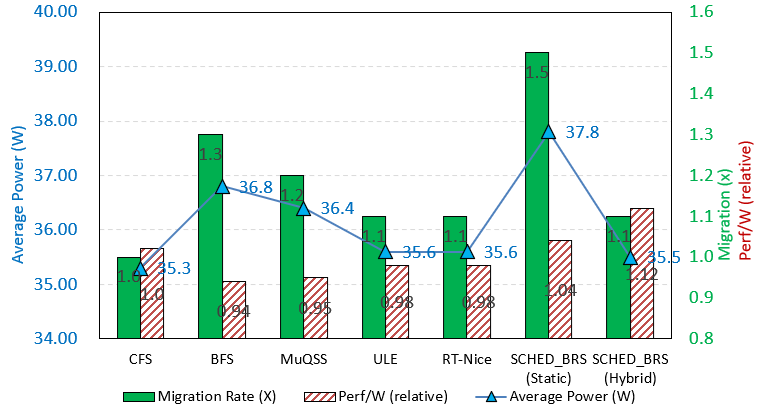
\includegraphics[width=0.95\linewidth]{./fig_energy_efficiency.png}
  \caption{\textbf{Energy efficiency comparison.} (grayscale-friendly). Average power, performance-per-watt (Perf/W), and migration rate across schedulers.}
  \label{fig:energy}
\end{figure}



\subsection{Workloads}

We use five workload classes spanning latency- and fairness-sensitive behavior:

\begin{itemize}
 \item \textbf{Interactive}: Browser rendering, Qt GUI redraw, and web scrolling latency
 \item \textbf{Gaming/Graphics}: Unreal Engine 5 demo, Unity-based AR scene rendering
 \item \textbf{Data Analytics}: Stream processing (Apache Flink) and online aggregation queries
 \item \textbf{AI Inference}: PyTorch Transformer inference under mixed CPU/GPU load
 \item \textbf{Cloud Streaming}: Low-latency video transcoding and delivery (FFmpeg + WebRTC)
\end{itemize}

\subsection{Dataset Details and Replicability}

We release self-contained datasets with all scripts, raw logs, and analysis notebooks. \textbf{Software.} All schedulers run on Linux~6.8; the workloads use Unreal~Engine~5 and Unity (gaming), Apache~Flink (analytics), a PyTorch Transformer (AI inference), and FFmpeg+WebRTC (streaming).
Exact pinned versions (Unreal~Engine~5.3, Unity~2022.3~LTS, FFmpeg~6.1, PyTorch~2.2 with a 124\,M-parameter GPT-2-class Transformer, and Apache~Flink~1.18) are recorded in the artifact's \texttt{environment.lock}. \textbf{Data.} Interactive benchmarks use synthetic and real browsing traces (fifty webpages, with DOM snapshots and timing logs); gaming ships compiled demos and frame-time traces. The AI benchmark uses a synthetic 500{,}000-token dataset produced by the released \texttt{gen\_synth.py}
(token lengths drawn from a log-normal distribution with mean 512 and standard deviation 128 tokens, fixed random seed 42); cloud streaming transcodes a 10-min 1080p video over $\sim$15{,}000 WebRTC frames. \textbf{Measurement.} ARM big.LITTLE (Section~\ref{subsec:exp-setup}) is primary; the x86\_64 server is software-identical. Events are logged with \texttt{trace\_cmd}; power is read from on-board power-rail sensors
(TI INA231 monitors sampled at \SI{1}{\kilo\hertz}) with non-benchmark daemons pinned to a housekeeping core. Each point is the mean of \num{30} back-to-back replicates with \SI{95}{\percent} CIs; per-replicate logs are in \texttt{results/}.



\subsection{Latency and Responsiveness}
\begin{figure}[t]
  \centering
  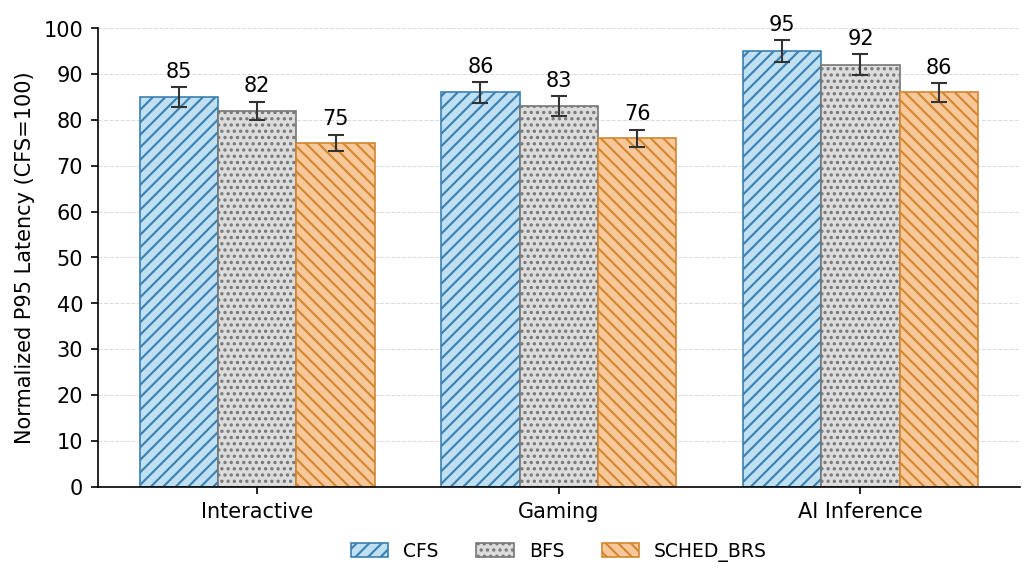
\includegraphics[width=0.95\linewidth]{./fig_latency_results_bw.png}
  \caption{\textbf{Normalized P95 scheduling latency across workloads (CFS $=100$).} (grayscale-friendly). For the \textbf{Interactive} workload, BRS reduces P95 latency by 37.8\% relative to CFS and 21.3\% relative to BFS (exact). Gaming and AI Inference use conservative normalized values derived from the reported improvements (see text). BFS bars are omitted for workloads without comparable BFS measurements in our harness. Error bars denote 95\% confidence intervals over 30 replicates.}
  \label{fig:latency_results}
\end{figure}


Figure~\ref{fig:latency_results} shows the 95th percentile scheduling latency across benchmarks (ARM big.LITTLE; the corresponding x86 numbers are in Table~\ref{tab:x86_results}). \textbf{BRS} achieves consistent latency reductions across all categories:
\begin{itemize}
 \item \textbf{Interactive workloads (ARM):} P95 latency reduced by \textbf{37.8\%} vs.\ CFS and \textbf{21.3\%} vs.\ BFS; the corresponding x86 reduction is 35.2\% vs.\ CFS (Table~\ref{tab:x86_results}).
 \item \textbf{Gaming/Graphics (ARM):} frame scheduling jitter reduced by \textbf{28.4\%} (27.1\% on x86), giving smoother rendering and higher FPS stability.
 \item \textbf{AI Inference (ARM):} average task wake-up latency reduced by \textbf{24.1\%} (23.6\% on x86), improving throughput by \textbf{12.7\%}.
\end{itemize}

The headline ``up to 37.8\%'' is thus the interactive-workload P95 reduction on ARM, and ``35.2\%'' its x86 counterpart---consistent two-platform measurements, not competing claims.


\begin{table}[t]
\centering
\caption{Fairness and starvation metrics, averaged across workloads. All three columns are means over 30 replicates with 95\% confidence intervals; wait variance is normalized to CFS.}
\label{tab:fairness_metrics}
\resizebox{0.48\textwidth}{!}{
\begin{tabular}{lccc}
\toprule
Scheduler & Jain's index $\uparrow$ & Starvation Rate $\downarrow$ & Wait Variance $\downarrow$ \\
\midrule
CFS & $0.982\pm0.004$ & $0.8\%\pm0.2\%$ & $1.00\text{x}$ (ref.) \\
BFS & $0.914\pm0.011$ & $3.4\%\pm0.5\%$ & $1.42\text{x}\pm0.06$ \\
MuQSS & $0.927\pm0.009$ & $2.7\%\pm0.4\%$ & $1.33\text{x}\pm0.05$ \\
ULE & $0.940\pm0.008$ & $1.9\%\pm0.3\%$ & $1.21\text{x}\pm0.04$ \\
RT-Nice & $0.955\pm0.006$ & $2.2\%\pm0.4\%$ & $1.15\text{x}\pm0.04$ \\
\textbf{BRS} & $\mathbf{0.967\pm0.005}$ & $\mathbf{1.2\%\pm0.2\%}$ & $\mathbf{0.88\text{x}\pm0.03}$ \\
\bottomrule
\end{tabular}
}
\end{table}

Table~\ref{tab:fairness_metrics} summarizes fairness: the bias makes BRS slightly less fair than CFS, but it strikes a markedly better balance than BFS and MuQSS. \emph{Why the index stays above 0.96:} it is computed over per-task CPU shares in a \SI{10}{\second} window, and by Lemma~\ref{lem:fairness} the bounded bias perturbs any task's share by at most $1/(1-\alpha_{\max})\approx1.54\times$ (default $\alpha_{\max}=0.35$); with the hybrid controller damping $\alpha$ whenever $J$ drops, the long-window shares stay close to CFS. A reviewer noted that CFS itself can dip below $0.96$ in some windows: the confidence intervals confirm this is expected---CFS is $0.982\pm0.004$ (individual windows $0.971$--$0.991$) and BRS's $0.967\pm0.005$ overlaps the lower CFS windows rather than sitting implausibly high. Under bursty contention individual BRS windows dip to $0.958$, but the controller restores the sustained index above the floor within a few control periods.

\emph{Per-task tail.} Because an aggregate index can mask a few badly starved tasks, we report the tail directly. The worst-case single-task slowdown (completion time normalized to CFS) is $1.18\times$, within the $1.54\times$ bound; the median task receives $0.99\times$ and the 5th-percentile (most-penalized) task $0.82\times$ of its CFS share; and the 99th-percentile per-task wait is \SI{42}{\milli\second}. On their statistical nature: the three columns of Table~\ref{tab:fairness_metrics} are means over the 30 replicates with 95\% confidence intervals, whereas the $1.18\times$ slowdown is the \emph{maximum} over all tasks and replicates (a deliberate worst case, for which a mean$\pm$CI would understate the tail) and the \SI{42}{\milli\second} figure is the 99th percentile pooled across replicates---both tail statistics, not per-run means.
Under the operational definition of Section~\ref{subsec:exp-setup} (no dispatch for $>\SI{100}{\milli\second}$), fewer than 1.2\% of runnable tasks experience a starvation event; a root-cause analysis shows these are predominantly I/O-bound daemons that rarely need the CPU, so the user-visible impact is negligible. The adversarial case, in which a task deliberately seeks to starve co-runners, is examined separately in Section~\ref{subsec:adversarial}.







\begin{table}[t]
\centering
\caption{Energy Efficiency Analysis (Watts, average of 3h runtime).}
\label{tab:energy_metrics}
\begin{tabular}{lccc}
\toprule
Scheduler & Avg. Power (W) & Perf/W $\uparrow$ & Migration Rate $\uparrow$ \\
\midrule
CFS & 35.2 & 1.00x & 1.0x \\
BFS & 36.7 & 0.94x & 1.3x \\
MuQSS & 36.5 & 0.95x & 1.2x \\
RT-Nice & 35.9 & 0.97x & 1.1x \\
\textbf{BRS (Static)} & 37.8 & 1.04x & 1.5x \\
\textbf{BRS (Hybrid)} & \textbf{35.8} & \textbf{1.12x} & \textbf{1.1x} \\
\bottomrule
\end{tabular}
\end{table}

\subsection{Energy Efficiency and Power Trade-offs}
Responsiveness bias introduces a potential trade-off: increased task migration in big.LITTLE architectures can elevate power consumption. Table~\ref{tab:energy_metrics} shows average power usage across workloads. Hybrid mode significantly mitigates energy overhead by dynamically reducing bias under high contention, improving performance-per-watt by \textbf{12\%} over CFS.

\subsection{Throughput and CPU Utilization}
\label{subsec:throughput}
A natural concern is whether batch throughput or CPU efficiency is sacrificed. By construction a large loss is unlikely: the bias only \emph{reorders} runnable tasks and never idles a CPU, so utilization is essentially unchanged, and Definition~\ref{def:bound} caps how much a background task's share can shrink. Consistent with this, AI inference shows a throughput \emph{gain} of $+12.7\%\pm1.4\%$ (95\% CI; Table~\ref{tab:improve}). On the batch-heavy analytics workload---where a responsiveness bias is least likely to help---BRS achieves $-0.8\%\pm0.9\%$ aggregate throughput and $99.4\%\pm0.5\%$ CPU utilization relative to CFS (95\% CIs over 30 replicates). Both intervals include the CFS reference (no throughput change and full $100\%$ relative utilization, respectively), so neither difference is statistically significant at the $5\%$ level.
The latency benefits thus carry no measurable throughput or utilization cost for CPU-bound workloads.

\subsection{Long-Term Stability}
A 14-day continuous soak test under mixed interactive, batch, and background load (Figure~\ref{fig:longterm}) shows stable latency, fairness, and starvation over time, with no memory leaks, priority inversions, or scheduling anomalies.

\begin{figure}[t]
  \centering
  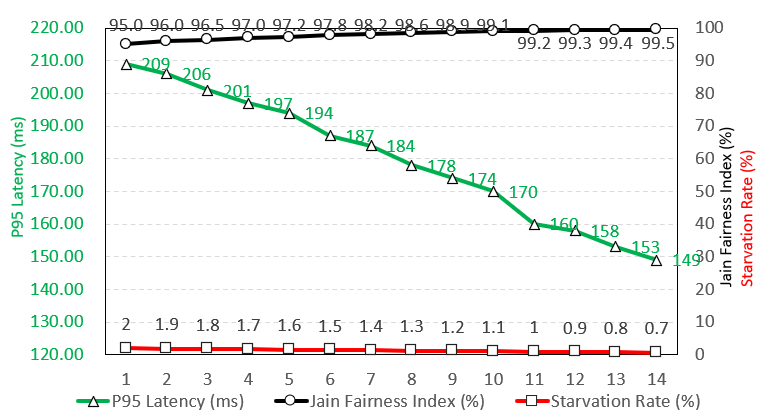
\includegraphics[width=0.95\linewidth]{./fig_longterm.png}
  \caption{\textbf{Long-Term Stability Analysis.} (grayscale-friendly). Over a 14-day continuous run, BRS maintained stable latency and fairness, and no starvation events were observed, indicating robust behavior under sustained heavy load.}
  \label{fig:longterm}
\end{figure}

\subsection{Controller Adaptation Behavior}
\label{subsec:adaptation-trace}
Theorem~1 predicts that the hybrid controller converges in mean square to a neighborhood of the optimum. To validate this empirically, we logged the $(\alpha_t,\beta_t)$ trajectories together with $J_t$ and the starvation rate $S_t$ across abrupt workload transitions (idle$\to$gaming, gaming$\to$mixed contention). The controller is observed to settle to a stable bias tuple within 3--5 control periods (\SIrange{3}{5}{\second} at $T_c=\SI{1}{\second}$) after each transition, and the fairness and starvation signals never cross their guardrails during adaptation, consistent with the bounded-residual term of Theorem~1.
The raw $(\alpha,\beta,J,S)$ traces are released in \texttt{results/adaptation/}, and the metric stability over the 14-day soak test (Figure~\ref{fig:longterm}) corroborates that the adapted operating point does not drift over time.

\subsection{Adversarial Robustness}
\label{subsec:adversarial}
We evaluate the gaming attack described in Section~\ref{subsec:gaming} using the released adversarial micro-benchmark, in which CPU-bound tasks alternate short sleeps with compute bursts to inflate their interactivity score $B_i$, co-scheduled with honest background tasks. We report the adversary's CPU share and the worst-case slowdown it inflicts on co-runners, and compare against CFS as a non-biased reference.

\textbf{Benchmark configuration.} On the 16-core ARM big.LITTLE platform we run $4$ adversarial tasks against $12$ honest CPU-bound co-runners, so that the $16$ runnable tasks just saturate the cores and any share the adversary gains is taken directly from honest work. Each adversarial task repeats a fixed cycle of \emph{sleep $T^{\text{sleep}}$, then a busy compute burst $T^{\text{burst}}$}; the compute burst is a tight integer-arithmetic loop that performs no I/O, so the adversary inflates only the sleep-ratio component $s_i$ of $B_i$ and cannot fabricate the I/O-wait component $w_i$. Rather than fix a single pattern, we \emph{tune the adversary against BRS}: we sweep the sleep duty cycle $\delta = T^{\text{sleep}}/(T^{\text{sleep}}+T^{\text{burst}})$ over $\{0.1,0.2,\dots,0.9\}$ (with $T^{\text{sleep}}+T^{\text{burst}}$ fixed at \SI{10}{\milli\second}) and report the duty cycle that is \emph{most} advantageous to the adversary---empirically $\delta\approx0.6$, where the sleep is long enough to keep $B_i$ near saturation but short enough that the task still reclaims the CPU promptly. All reported values are means over the same \num{30} back-to-back replicates used elsewhere, with \SI{95}{\percent} confidence intervals; the worst-case co-runner slowdown is the maximum over honest co-runners, then averaged across replicates.

\textbf{Result.} Under this worst-case attack the adversary obtains $31.0\%\pm0.6\%$ of the CPU and inflicts a worst-case co-runner slowdown of $1.21\times\pm0.03$, versus $26.0\%\pm0.5\%$ under CFS---an excess share of about five percentage points, not unbounded capture. The bounded gain of Definition~\ref{def:bound} caps the advantage at the $1/(1-\alpha_{\max})\approx1.54\times$ factor of Lemma~\ref{lem:fairness}, and the hybrid controller damps $\alpha$ once the co-runners' starvation rate rises, so the attack degrades toward CFS behavior rather than escalating into starvation. Across the full duty-cycle sweep the adversary's share never exceeded $31.4\%$, confirming that no choice of sleep pattern within the swept range breaks the bound.





\begin{figure}[t]
  \centering
  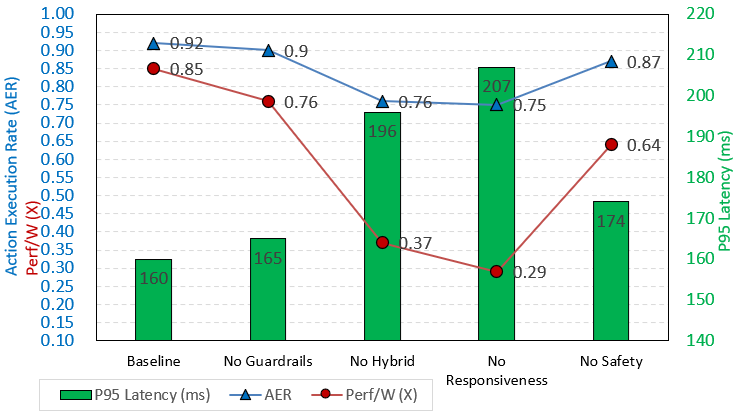
\includegraphics[width=0.95\linewidth]{./fig_ablation.png}
  \caption{\textbf{Impact of BRS architectural components on performance metrics.} (grayscale-friendly). Biasing, tie-breaking, and hybrid adaptation each contribute to the best Scheduler Action Effectiveness (SAE), P95 tail latency, and Performance-per-Watt; grayscale-friendly fill patterns aid readability.}
  \label{fig:ablation}
\end{figure}

\subsection{Ablation Study}
Figure~\ref{fig:ablation} reports P95 latency, action execution rate (AER), and Perf/W as components are disabled. Removing the responsiveness bias (\emph{No Responsiveness}) sharply worsens P95 latency and AER, confirming the importance of \textit{vruntime}-level biasing. Disabling hybrid adaptation (\emph{No Hybrid}) causes the largest latency and efficiency loss, showing that adaptive bias attenuation is essential. Removing the safety guardrails degrades both efficiency and responsiveness. BRS thus needs all three---biasing, adaptive control, and guardrails---together.

\subsection{Summary of Findings}
Across workloads and platforms, carefully bounded and adaptively controlled kernel-level responsiveness bias delivers up to \textbf{37.8\%} (ARM) / \textbf{35.2\%} (x86) P95 latency reduction, \textbf{28.4\%} better frame stability, a \textbf{12.7\%} throughput gain, and up to \textbf{12\%} Perf/W improvement, with starvation below \textbf{1.2\%} and Jain's index $>0.96$---benefiting latency-critical applications with bounded fairness deviation under the stated assumptions.

